\chapter{Advanced Tie Points}



%=======================================================================================================
\section{Tie points on low contrast images}


The current implementation of SIFT++ used in MicMac is not fully invariant to scaling/translation in radiometry. This may be a problem in case of acquisitions having a good SNR but with low contrast in the scene; in this case, thanks to good SNR there is potential information to get tie points, but as this information is assimilated to noise, it cannnot be extracted.

To overcome this problem, it is possible to require that MicMac computes some contrast enhancement on images before computing SIFT points. Although this method is not optimal (it would be better to modify the SIFT++ Kernel), it has the advantage of existing\dots



The figure~\ref{FIG:SF:Det} presents an image without enhancement, in its original form, and the same image after enhancement. The figure~\ref{FIG:SF:TieP} presents the detected tie points; we notice that the spatial density of tie points is much higher on enhanced image.

Of course, the enhanced images are fairly artificial, as it can be seen on figure~\ref{FIG:SF:Img} that presents a full image before and after enhancement. So if this option is activated, the enhanced images are used only for the tie points steps (which are developed as specific "hidden files" in folder {\tt Tmp-MM-Dir}).


To activate this option, the {\tt NKS-Assoc-SFS} must be changed in the {\tt MicMac-LocalChantierDescripteur.xml}. It must return {\tt SFS} instead of the default value {\tt NONE}. For example:

\begin{verbatim}
    <KeyedNamesAssociations>
        <Calcs>
            <Arrite>  1 1 </Arrite>
            <Direct>
                <PatternTransform> .* </PatternTransform>
                <CalcName>  SFS </CalcName>
            </Direct>
        </Calcs>
        <Key>   NKS-Assoc-SFS </Key>
    </KeyedNamesAssociations>
\end{verbatim}

\begin{figure}
\begin{center}
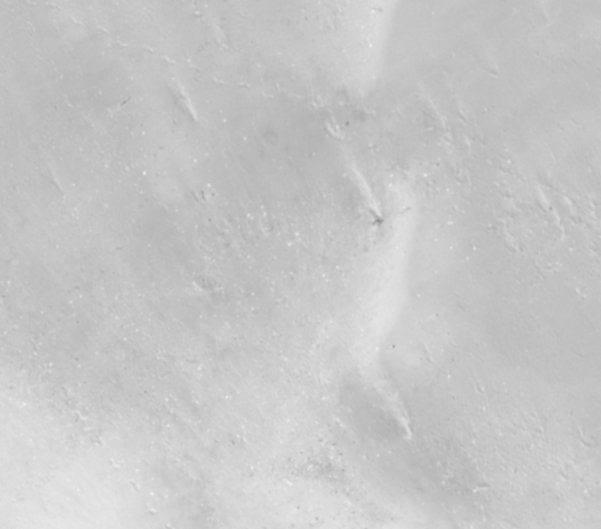
\includegraphics[width=0.4\textwidth]{FIGS/Tapioca-SFS/Detail-STD.jpg}
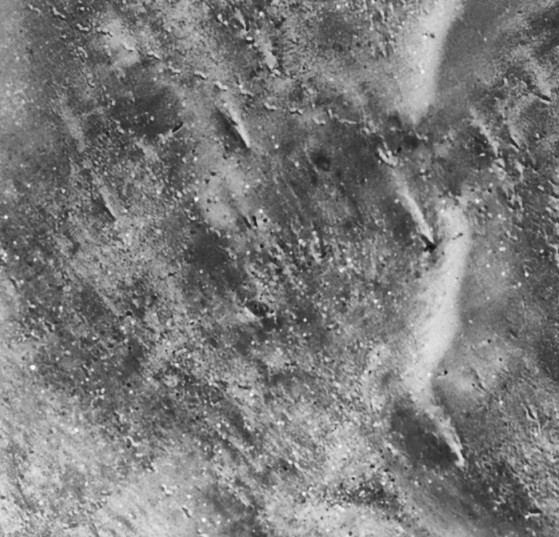
\includegraphics[width=0.4\textwidth]{FIGS/Tapioca-SFS/Detail-SFS.jpg}
\end{center}
\caption{Detail of image before and after enhancement}
\label{FIG:SF:Det}
\end{figure}


\begin{figure}
\begin{center}
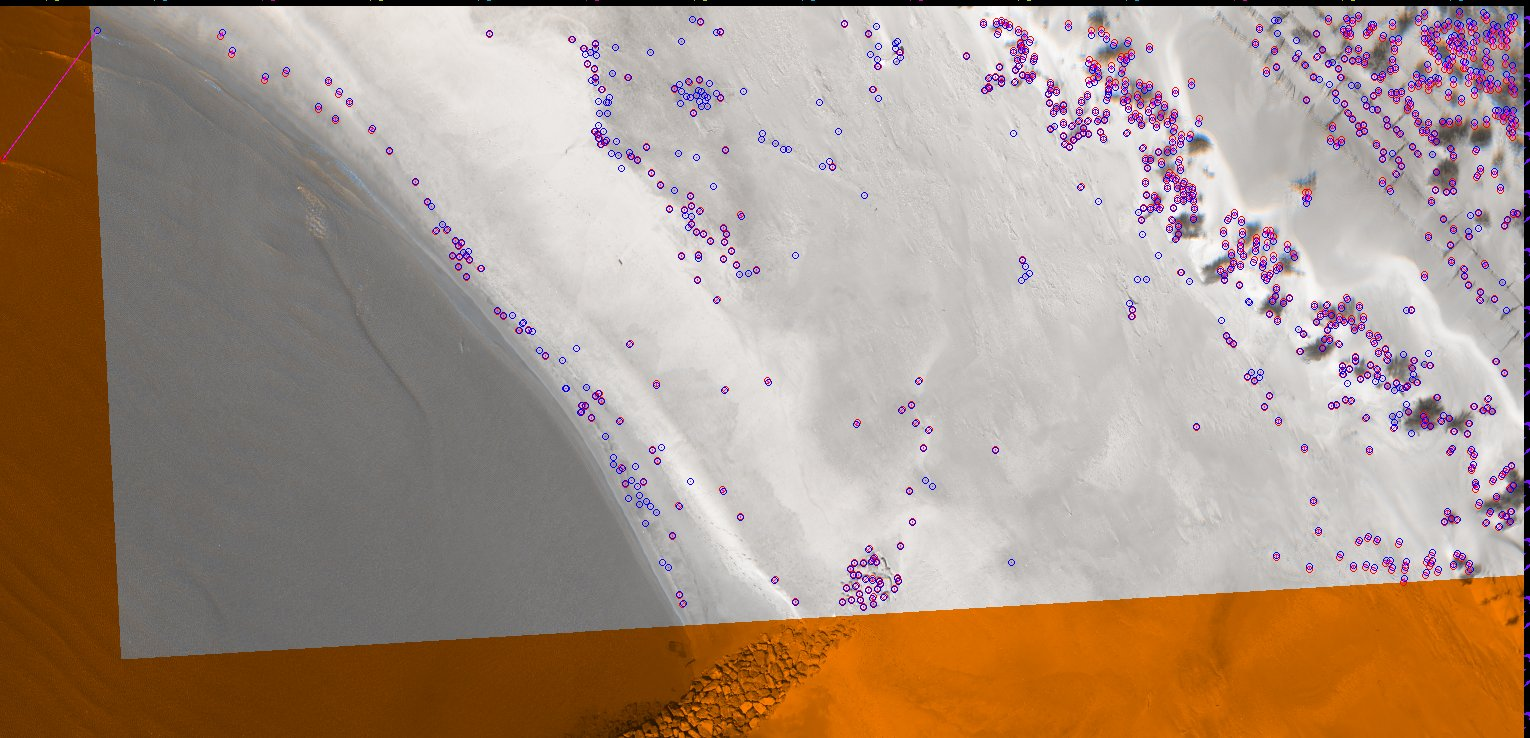
\includegraphics[width=0.95\textwidth]{FIGS/Tapioca-SFS/SIFT-STD.jpg}
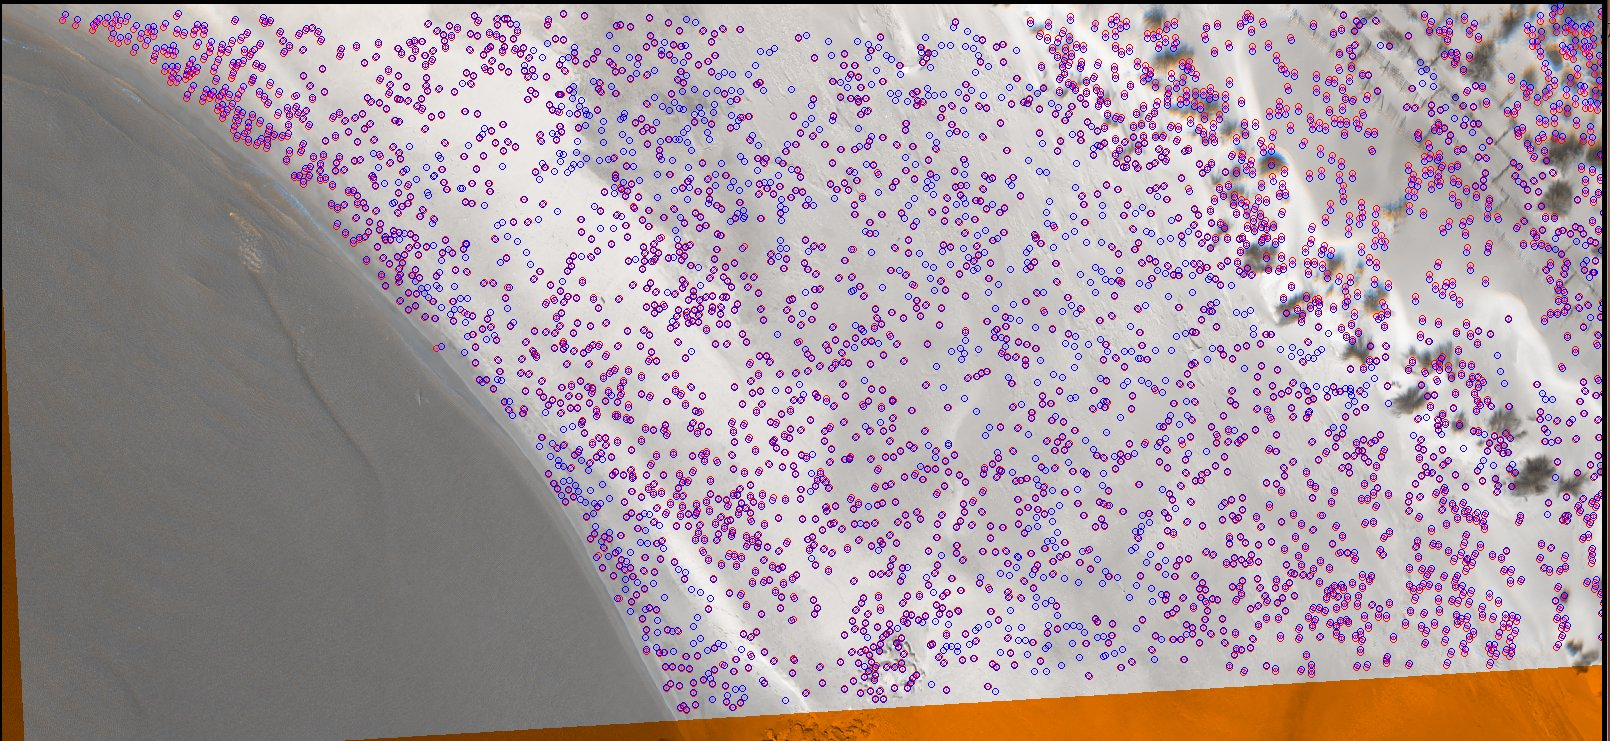
\includegraphics[width=0.95\textwidth]{FIGS/Tapioca-SFS/SIFT-SFS.jpg}
\end{center}
\caption{Tie points before and after enhancement}
\label{FIG:SF:TieP}
\end{figure}

\begin{figure}
\begin{center}
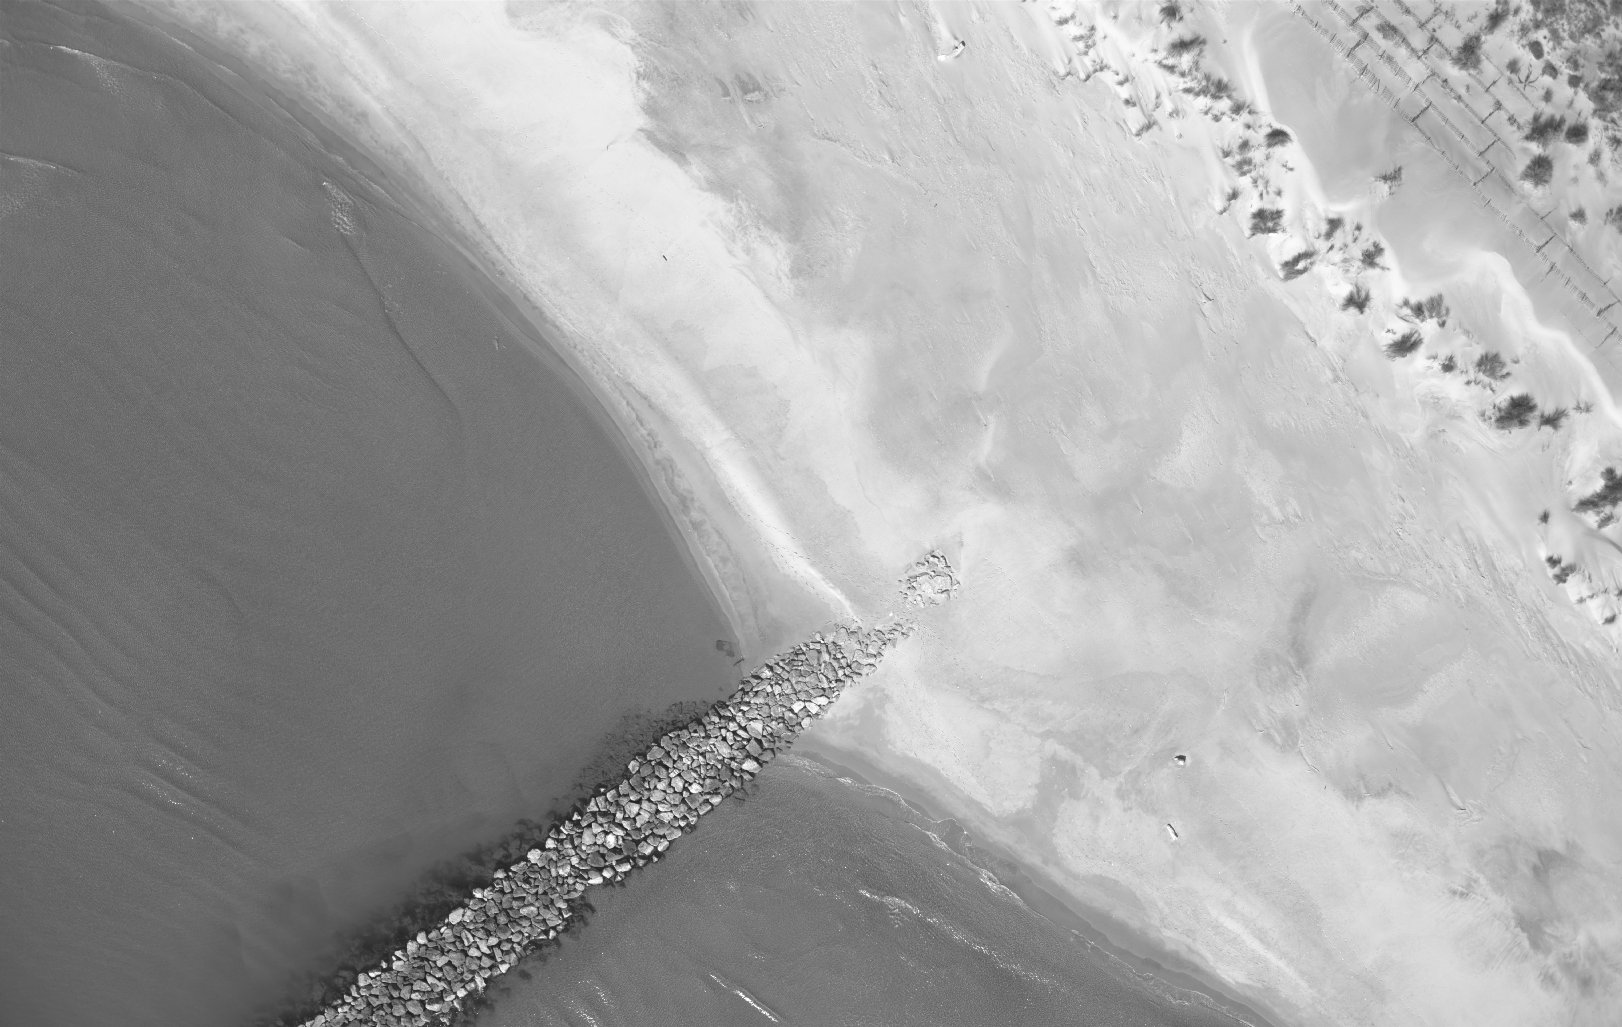
\includegraphics[width=0.95\textwidth]{FIGS/Tapioca-SFS/Im-STD.jpg}

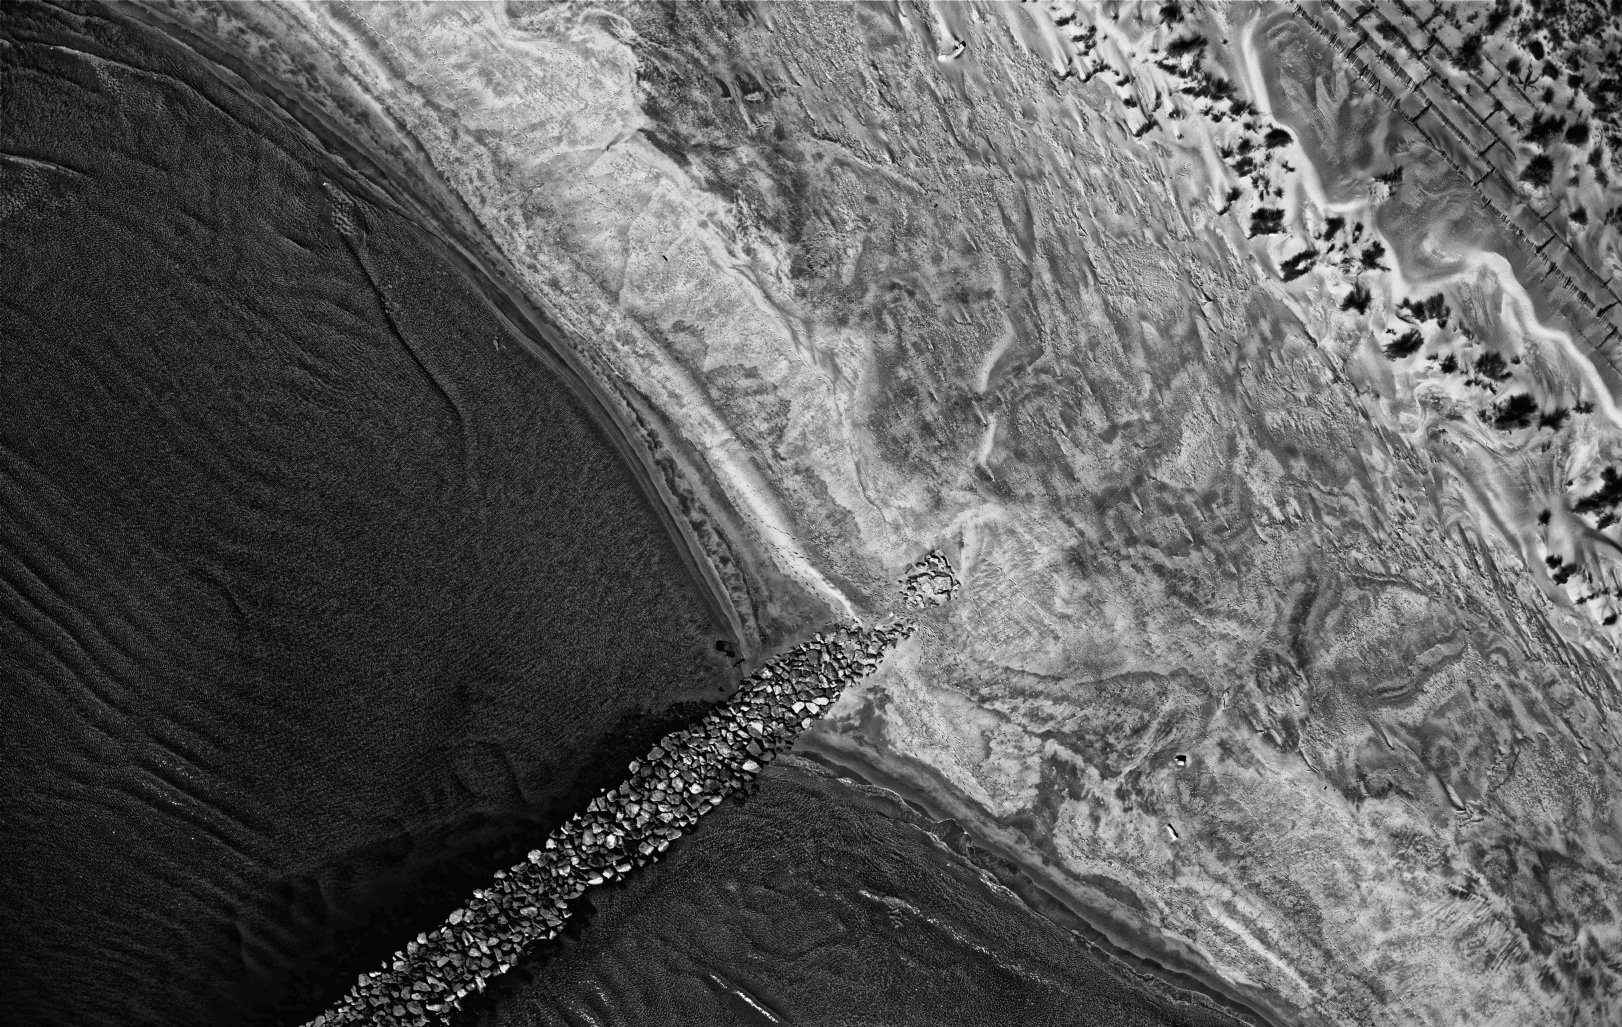
\includegraphics[width=0.95\textwidth]{FIGS/Tapioca-SFS/Im-SFS.jpg}
\end{center}
\caption{Global images before and after enhancement}
\label{FIG:SF:Img}
\end{figure}



